\documentclass{article}
\usepackage{tikz}
\usetikzlibrary{knots,hobby}

\begin{document}
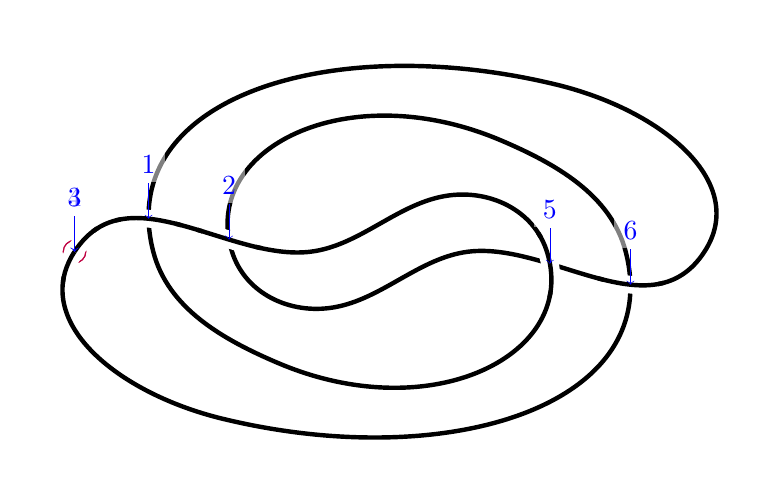
\begin{tikzpicture}[use Hobby shortcut]
\begin{knot}[
  consider self intersections,
  draft mode=crossings,
  ignore endpoint intersections=false,
  every strand/.style={draw,ultra thick},
  clip width=4,
  flip crossing/.list={4}
]
\strand ([closed]-4,0) .. (-1,0) .. (45:1).. (0:2) .. (-135:2) .. (180:3) .. (45:3) .. (0:4) .. (0:1) .. (-135:1) .. (180:2) .. (45:2) .. (0:3) .. (-135:3);
\end{knot}
\end{tikzpicture}

%\begin{tikzpicture}
%\draw[ultra thick] (.5,0) -- (3,0);
%\draw[ultra thick] (1,0) arc [start angle=0, end angle=180, radius=1];
%\draw[ultra thick] (2,0) arc (0:180:2);
%\draw[ultra thick] (3,0) arc (0:180:3);
%
%\end{tikzpicture}


\end{document}

%  controls +(1,0) and +(-1,0) ..